% Formula sheet for MEC E 371 Heat Transfer
% Two column format

\documentclass[10pt]{article}
\usepackage{amsmath}
\usepackage{amssymb}
\usepackage{multicol}
\usepackage{geometry}
\usepackage{fancyhdr}
\usepackage{siunitx}
\usepackage{enumitem}
\usepackage{multicol}
\usepackage{graphicx}
\usepackage{multirow}
\usepackage{lastpage}
\usepackage[final]{hyperref}
\usepackage{parskip}
\usepackage{float}
\usepackage{subcaption}

\geometry{letterpaper, portrait, margin=0.5in, footskip=0.25in, top = 0.75in, headsep=0.25in}
\setlength{\columnsep}{0.5in}

\hypersetup{
	colorlinks=true,       % false: boxed links; true: colored links
	linkcolor=blue,        % color of internal links
	citecolor=blue,        % color of links to bibliography
	filecolor=magenta,     % color of file links
	urlcolor=blue         
}

\pagestyle{fancy}
\fancyhf{}
\lhead{MEC E 371 Formula Sheet}
\chead{Last Updated: \today}
\rhead{Alex Diep}
\cfoot{\thepage\ of \pageref{LastPage}}

\begin{document}
%\maketitle
%\thispagestyle{empty}
\setlength{\belowdisplayskip}{4pt} \setlength{\belowdisplayshortskip}{0pt}
\setlength{\abovedisplayskip}{4pt} \setlength{\abovedisplayshortskip}{0pt}
\begin{multicols*}{2}
\section*{8. Internal Forced Convection}
\subsection*{8.1. General Procedure}
\begin{enumerate}
    \item Find fluid properties from Appendix 1 at bulk mean temperature $T_b = (T_i + T_e)/2$
    \begin{itemize}
        \item $\rho$, $\mu$, $k$, $c_p$, $Pr$, $\nu$
    \end{itemize}
    \item Determine mean velocity $V_{\text{avg}}$
    \item Determine the type of flow (laminar or turbulent)
    \begin{itemize}
        \item Laminar: Re $< 2300$
        \item Turbulent: Re $> 4000$
    \end{itemize}
    \item Determine the Nusselt number, Nu, using the appropriate correlation
    \begin{itemize}
        \item Check if $l_{h, \text{laminar}}$ and $l_{t, \text{laminar}}$ is less than $L$. If so, use Table \ref{tab:sec8_fully_developed_laminar} 
        \item Else, use empirical correlations
    \end{itemize}
    \item Determine the heat transfer coefficient $h$ using $Nu$, $k$, and $A_s$
\end{enumerate}

% Add this to a glossary section later
\subsection*{8.2. Variable Definitions}
\begin{itemize}
    \item Nu: Nusselt number
    \item Re: Reynolds number
    \item Pr: Prandtl number
    \item $\mu$: Dynamic viscosity
    \item $\nu$: Kinematic viscosity
    \item $k$: Thermal conductivity
    \item $h$: Convection heat transfer coefficient
    \item $D_h$: Hydraulic diameter
    \item $A_s$: Surface area
    \item $A_c$: Cross-sectional area
    \item $V_{\text{avg}}$: Average velocity
    \item $T_b$: Bulk mean temperature
    \item $T_i$: Inlet temperature
    \item $T_e$: Exit temperature
    \item $\dot{m}$: Mass flow rate
    \item $\dot{q}$: Heat flux 
    \item $\Delta T_{\text{lm}}$: Log mean temperature difference   
\end{itemize}

\subsection*{8.3. Formulas}
\subsubsection*{8.3.1. General Formulas}
\begin{align*}
    \dot{m} &= \rho V_{\text{avg}} A_c \\
    \text{Re} &= \frac{\rho V_{\text{avg}} D_h}{\mu}  = \frac{V_{\text{avg}} D_h}{\nu} \\
    D_h &= \frac{4 A_c}{\text{Perimeter}} = D\rvert_{\text{circular}} = a\rvert_{\text{square}}   \\
    &= \frac{2ab}{a + b} \bigg\rvert_{\text{rectangular}} = \frac{4ab}{a+b}\bigg\rvert_{\text{channel}} \\
    \text{Nu} &= \frac{hD_h}{k} \\ 
    A_s &= \pi D L|_{\text{circular}} = 4ab|_{\text{rectangular}} \\
    A_c &= \pi \frac{D^2}{4}|_{\text{circular}} = ab|_{\text{rectangular}} \\
    l_{h, \text{laminar}} &= 0.05 \text{Re} D_h \\
    l_{t, \text{laminar}} &= 0.05 \text{Re} \text{Pr} D_h = \text{Pr} l_{h, \text{laminar}} \\
    l_{h, \text{turbulent}} &\approx l_{t, \text{turbulent}} = 10D_h 
\end{align*}
\subsubsection*{8.3.2. Constant $\dot{q}$}
\begin{align*}
    T_e &= T_i + \frac{\dot{q}}{\dot{m} c_p} \\ 
    \dot{q} &= h(T_s-T_b)
\end{align*}
\subsubsection*{8.3.3. Constant $T_s$}
\begin{align*}
    T_e &= T_s - (T_s - T_i) \exp\left(-\frac{h A_s}{\dot{m} c_p}\right) \\
    T_s &=\frac{T_e - T_i \exp\left(-\frac{\dot{m} C_p}{h A_s}\right)}{1 - \exp\left(-\frac{\dot{m} C_p}{h A_s}\right)} \\
    \dot{Q} &= h A_s \Delta T_{\text{lm}} \\
    T_{\text{lm}} &= \frac{T_{i} - T_{e}}{\ln[(T_{s} - T_{e})/(T_{s} - T_{i})]} 
\end{align*}    
\subsubsection*{8.3.4. Correlations for Nu}
For fully developed laminar flow, use Table \ref{tab:sec8_fully_developed_laminar}.

For entry region in a circular tube where $T_s = \text{constant}$, use:
\begin{align*}
    \text{(Edwards et al., 1979) } \text{Nu} = 3.66 + \frac{0.0658(D/L) \text{Re} \text{Pr}}{1 + 0.04[(D/L) \text{Re} \text{Pr}]^{2/3}} 
\end{align*}

For entry region in a circular tube where the difference between $T_s$ and $T_b$ is large, use:
\begin{align*}
    \text{(Sieder and Tate, 1936) } &\text{Nu} = 1.86\left(\frac{\text{Re} \text{Pr} D}{L}\right)^{1/3} \left(\frac{\mu_b}{\mu_s}\right)^{0.14} \\
    0.6 < \text{Pr} < 5, &\quad 0.0044 < \frac{\mu_b}{\mu_s} < 9.75
\end{align*}
All properties for Sieder and Tate should be evaluated at $T_b$ except $\mu_s$ which should be evaluated at $T_s$.

For entry region between two isothermal parallel plates, use:
\begin{align*}
    \text{(Edwards et al., 1979) } &\text{Nu} = 7.54 + \frac{0.03(D_h/L) \text{Re} \text{Pr}}{1 + 0.016[(D_h/L) \text{Re} \text{Pr}]^{2/3}} \\
    &\text{Re} \leq 2800
\end{align*}
For turbulent flow in a circular tube, use:
\begin{align*}
    \text{(Dittus-Boelter, 1930) } \text{Nu} = 0.023 \text{Re}^{0.8} \text{Pr}^{n}  \\
    n = 0.4 \; (\text{Heating}), \quad n = 0.3 \; (\text{Cooling}) 
\end{align*}
% Pressure drop:\footnote{Check if $D_h$ should be used for $D$ in $V_{\text{avg}}$. Also I don't think he covers this in class.}
% \begin{align*}
%     \Delta P_{L} &= f \frac{L}{D_h} \frac{\rho V_{\text{avg}}^2}{2} \\
%     h_L &= \frac {\Delta P_L}{\rho g} = f \frac{L}{D_h} \frac{V_{\text{avg}}^2}{2g} \\
%     f|_{\text{laminar}} &= \frac{64}{\text{Re}} \\
%     V_{\text{avg}} &= \frac{\Delta P D^2}{32 \mu L} \\
% \end{align*} 
\end{multicols*}

\section*{Tables}
\begin{table}[H]
    \centering
    \caption{Nusselt number and friction factor for fully developed laminar flow in tubes of various cross sections 
    ($D_h = 4A_c /P$, $Re = V_{\text{avg}} D_h / \nu$, and $\text{Nu} = hD_h / k$) (\textbf{Table 8-1 in textbook})}
    \label{tab:sec8_fully_developed_laminar}
    \begin{tabular}{ccccc}
        \hline
        & & \multicolumn{2}{c}{Nu} & \\
        \cline{3-4}
        Tube Geometry & $a/b$ or $\theta^\circ$ & $T_s = \text{constant}$ & $\dot{q}_s = \text{constant}$ & $f$ \\
        \hline
        \raisebox{-\totalheight}{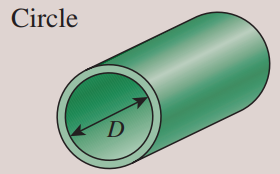
\includegraphics[width=0.15\textwidth]{Figures/Sec8 Circle Fully Laminar.png}} & --- & 4.36 & 3.66 & 64/Re \\
        \hline
        & \underline{$a/b$} & & & \\ 
        \multirow{2}{*}{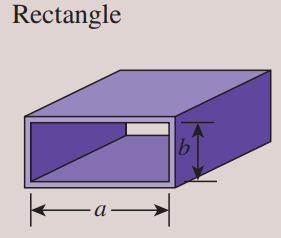
\includegraphics[width=0.15\textwidth]{Figures/Sec8 Rectangle Fully Laminar.png}} 
        & 1 & 2.98 & 3.61 & 56.92/Re \\
        & 2 & 3.39 & 4.12 & 62.20/Re \\
        & 3 & 3.96 & 4.79 & 68.36/Re \\
        & 4 & 4.44 & 5.33 & 72.92/Re \\
        & 6 & 5.14 & 6.05 & 78.80/Re \\
        & 8 & 5.60 & 6.49 & 82.32/Re \\
        & $\infty$ & 7.54 & 8.24 & 96.00/Re \\
        \hline
        & \underline{$a/b$} & & & \\
        \multirow{2}{*}{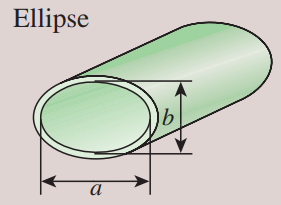
\includegraphics[width=0.15\textwidth]{Figures/Sec8 Ellipse Fully Laminar.png}}
        & 1 & 3.66 & 4.36 & 64.00/Re \\
        & 2 & 3.74 & 4.56 & 67.28/Re \\
        & 4 & 3.79 & 4.88 & 72.96/Re \\
        & 8 & 3.72 & 5.09 & 76.60/Re \\
        & 16 & 3.65 & 5.18 & 78.16/Re \\
        \hline
        & \underline{$\theta^\circ$} & & & \\
        \multirow{2}{*}{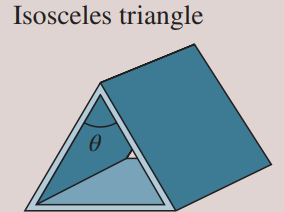
\includegraphics[width=0.15\textwidth]{Figures/Sec8 Triangle Fully Laminar.png}}
        & 10 & 1.61 & 2.45 & 50.80/Re \\
        & 30 & 2.26 & 2.91 & 52.28/Re \\
        & 60 & 2.47 & 3.11 & 53.32/Re \\
        & 90 & 2.34 & 2.98 & 52.60/Re \\
        & 120 & 2.00 & 2.68 & 50.96/Re \\
        \hline
        % \raisebox{-\totalheight}{\includegraphics[width=0.15\textwidth]{Figures/Sec8 Square Fully Laminar.png}} & 1 & 3.66 & 3.11 & 64/Re \\
    \end{tabular}
\end{table}
\newpage
\begin{multicols*}{2}
\section*{9. Natural Convection}
\subsection*{9.1. General Procedure}
\subsubsection*{9.1.1. Over Surfaces}
\begin{enumerate}
    \item Find Rayleigh number, Ra$_L$, using fluid properties at film temperature $T_f = (T_s + T_\infty)/2$
    \item Use the appropriate correlation in Table \ref{tab:sec9_natural_convection_over_surfaces} 
    to find the Nusselt number, Nu
    \item Determine the heat transfer coefficient $h$ using Nu, $k$, and $L_c$
\end{enumerate}
\subsubsection*{9.1.2. In Enclosures}
\begin{enumerate}
    \item Find Rayleigh number, Ra$_L$, using fluid properties at average temperature $T_{\text{avg}} = (T_1 + T_2)/2$
    where $T_1$ and $T_2$ are the temperatures of the hot and cold surfaces respectively.
    \item Use the appropriate correlation to find the Nusselt number, Nu
    \item Determine the heat transfer coefficient $h$ using Nu, $k$, and $L_c$
\end{enumerate}
% Add this to a glossary section later
\subsection*{9.2. Variable Definitions}
\begin{itemize}
    % \item Nu: Nusselt number
    % \item Re: Reynolds number
    % \item Pr: Prandtl number
    % \item $\mu$: Dynamic viscosity
    % \item $\nu$: Kinematic viscosity
    % \item $k$: Thermal conductivity
    % \item $h$: Convection heat transfer coefficient
    % \item $D_h$: Hydraulic diameter
    % \item $A_s$: Surface area
    % \item $A_c$: Cross-sectional area
    % \item $V_{\text{avg}}$: Average velocity
    % \item $T_b$: Bulk mean temperature
    % \item $T_i$: Inlet temperature
    % \item $T_e$: Exit temperature
    % \item $\dot{m}$: Mass flow rate
    % \item $\dot{q}$: Heat flux 
    % \item $\Delta T_{\text{lm}}$: Log mean temperature difference   
    \item Ra$_L$: Rayleigh number
    \item Gr$_L$: Grashof number
    \item $T_s$: Surface temperature
    \item $T_\infty$: Ambient temperature
    \item $T_f$: Film temperature
    \item $L_c$: Characteristic length
    \item $\beta$: Coefficient of volume expansion
    \item $\nu$: Kinematic viscosity
    \item $\alpha$: Thermal diffusivity
    \item $g$: Gravitational acceleration
\end{itemize}

\subsection*{9.3. Formulas}
\begin{align*}
    \text{Ra}_L &= \text{Gr}_L \text{Pr} = \frac{g \beta (T_s - T_\infty) L_c^3}{\nu^2} \text{Pr} \\
    \beta &= \frac{1}{T}, \quad \text{for ideal gases} \\
    h &= \frac{k \text{Nu}}{L_c} 
\end{align*}
\subsubsection*{9.3.1. Over Surfaces}
For convection 
\begin{align*}
    \dot{Q} &= h A_s (T_s - T_\infty)
\end{align*}
Use Table \ref{tab:sec9_natural_convection_over_surfaces} to find Nu.
\subsubsection*{9.3.2. In Rectangular Enclosures}
For convection in rectilinear enclosures, 
\begin{equation*}
    \dot{Q} = h A_s (T_1 - T_2) 
\end{equation*}
where $T_1$ and $T_2$ are the temperatures of the hot and cold surfaces respectively.

In \textbf{horizontal rectangular enclosures} ($L_c = L$, where $L$ is the gap between plates),
\begin{gather*}
    \text{Nu} = 1 + 1.44 \left[1 - \left(\frac{1708}{\text{Ra}_L}\right)\right]^{+} + \left[\frac{\text{Ra}_L}{18} - 1\right]^{+}\\
    \text{Ra}_L < 10^8 \; (\text{gases}), \quad \text{Ra}_L < 10^{5} \; (\text{liquids})
\end{gather*}
For large aspect ratios ($H/L \geq 12$), this equation (Hollands et al., 1976) correlates experimental data extremely well for tilt angles up to 70$^{\circ}$.
$\left[ \;\right]^+$ indicates that if the quantity in the bracket is negative, it should be set equal to zero.
\begin{gather*}
    \text{Nu}_L = 1 + 1.44 \left[1 - \left(\frac{1708}{\text{Ra}_L \cos\theta}\right)\right]^{+} + \left[\frac{\text{Ra}_L \cos\theta}{18} - 1\right]^{+}\\
    \text{Ra}_L < 10^8 \; (\text{gases}), \quad \text{Ra}_L < 10^{5} \; (\text{liquids}), \\
    0 < \theta < 70^{\circ}, \quad \frac{H}{L} \geq 12
\end{gather*}
In \textbf{vertical rectangular enclosures} ($L_c = L$, where $L$ is the gap between plates),
\begin{gather*}
    \text{Nu}_L = 0.18\left(\frac{\text{Pr}}{0.2 + \text{Pr}} \text{Ra}_L \right)^{0.29}\\
    \frac{\text{Pr}}{0.2 + \text{Pr}} > 10^3, \; 1 < \frac{H}{L} < 2 
\end{gather*}
or 
\begin{gather*}
    \text{Nu}_L = 0.22\left(\frac{\text{Pr}}{0.2 + \text{Pr}} \text{Ra}_L \right)^{0.28} \left(\frac{H}{L}\right)^{-0.25}\\
    \text{Ra}_L < 10^{10}, \; 2 < \frac{H}{L} < 10
\end{gather*}
or
\begin{gather*}
    \text{Nu}_L = 0.42\left(\frac{\text{Pr}}{0.2 + \text{Pr}} \text{Ra}_L \right)^{0.25}\text{Pr}^{0.012} \left(\frac{H}{L}\right)^{-0.3}\\
    1 < \text{Pr} < 2 \times 10^4, \; 10^4 < \text{Ra}_L < 10^7, \; 10 < \frac{H}{L} < 40
\end{gather*}
\subsubsection*{9.3.3. In Concentric Horizontal Cylinders}
In \textbf{concentric horizontal cylinders} ($L_c = (D_o - D_i)/2$, where $D_o$ and $D_i$ are the outer and inner diameters respectively),
\begin{equation*}
    \dot{Q}_{\text{cylinder}} = \frac{2\pi k \text{Nu}}{\ln(D_o/D_i)}(T_i - T_o) 
\end{equation*}
where $T_i$ and $T_o$ are the temperatures of the inner and outer surfaces respectively.
\begin{gather*}
    \text{Nu} = \max\left\{1, \;0.386 \left(\frac{\text{Pr}}{0.861 + \text{Pr}}\right)^{0.25}(F_{\text{cyl}} \text{Ra}_L)^{0.25}\right\}\\
    %\text{Nu} = \max\left{1, \right}
    %0.386 \left(\frac{\text{Pr}}{0.861 + \text{Pr}}\right)^{0.25}(F_{\text{cyl}} \text{Ra}_L)^{0.25}
%     F_{\text{cyl}} = \frac{\ln^4(D_o/D_i)}{L_{c}^3 (D_{i}^{-0.6}+D_{o}^{-0.6})^5} 
\end{gather*}
\subsubsection*{9.3.4. Combined Natural and Forced Convection}
For combined natural and forced convection, 
\begin{equation*}
    \text{Nu}_{\text{Overall}} = \left(\text{Nu}_{\text{Forced}}^n \pm \text{Nu}_{\text{Natural}}^n\right)^{1/n}
\end{equation*}
where the plus sign is for assisting flows and the minus sign is for opposing flows. $n = 3.5$ for 
horizontal plates and $n = 4$ for cylinders and spheres. Else use $n = 3$.
\end{multicols*}

\section*{Tables}
% \begin{table}[H]
%     \centering
%     \caption{Empirical correlations for the average Nusselt number for natural convection over surfaces 
%     (\textbf{Table 9-1 in textbook})}
%     \label{tab:sec9_natural_convection_over_surfaces}
%     \begin{tabular}{p{0.2\textwidth}p{0.1\textwidth}p{0.15\textwidth}p{0.4\textwidth}}
%         \hline
%         Geometry & Characteristic Length $L_c$ & Range & Nu \\
%         \hline
%         \multirow{2}{*}{Vertical Plate 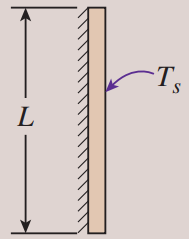
\includegraphics[width=0.1\textwidth]{Figures/Sec9 Vertical Plate.png}} 
%         & $L$ & $10^4 \leq \text{Ra}_L \leq 10^{9}$ & $\displaystyle \text{Nu} =0.59 \text{Ra}_L^{1/4}$ \\
%         & & $\displaystyle 10^{9} \leq \text{Ra}_L \leq 10^{13}$ & $\text{Nu} = 0.1 \text{Ra}_L^{1/3}$ \\
%         & & Entire range & $\displaystyle \text{Nu} = \left(0.825 + \frac{0.387 \text{Ra}_L^{1/6}}{[1 + (0.492/\text{Pr})^{9/16}]^{8/27}}\right)^2$ \\
%         & & & (complex but more accurate) \\
%         & & & \\
%         \hline
%         \multirow{2}{*}{Inclined Plate 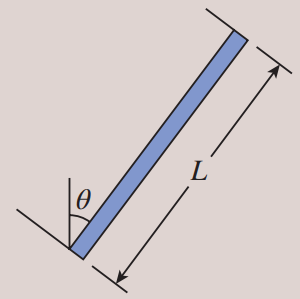
\includegraphics[width=0.1\textwidth]{Figures/Sec9 Inclined Plate.png}}
%         & $L$ & & Use vertical plate equations for the upper 
%         surface of a cold plate and the lower 
%         surface of a hot plate \\
%         & & & \\
%         & & & Replace $g$ with $g \cos\theta$ for $0 < \theta < 60^\circ$ \\
%         & & & \\
%         \hline
%         % finish later
%     \end{tabular}
% \end{table}
\begin{table}[H]
    \centering
    \caption{Empirical correlations for the average Nusselt number for natural convection over surfaces 
    (\textbf{Table 9-1 in textbook})}
    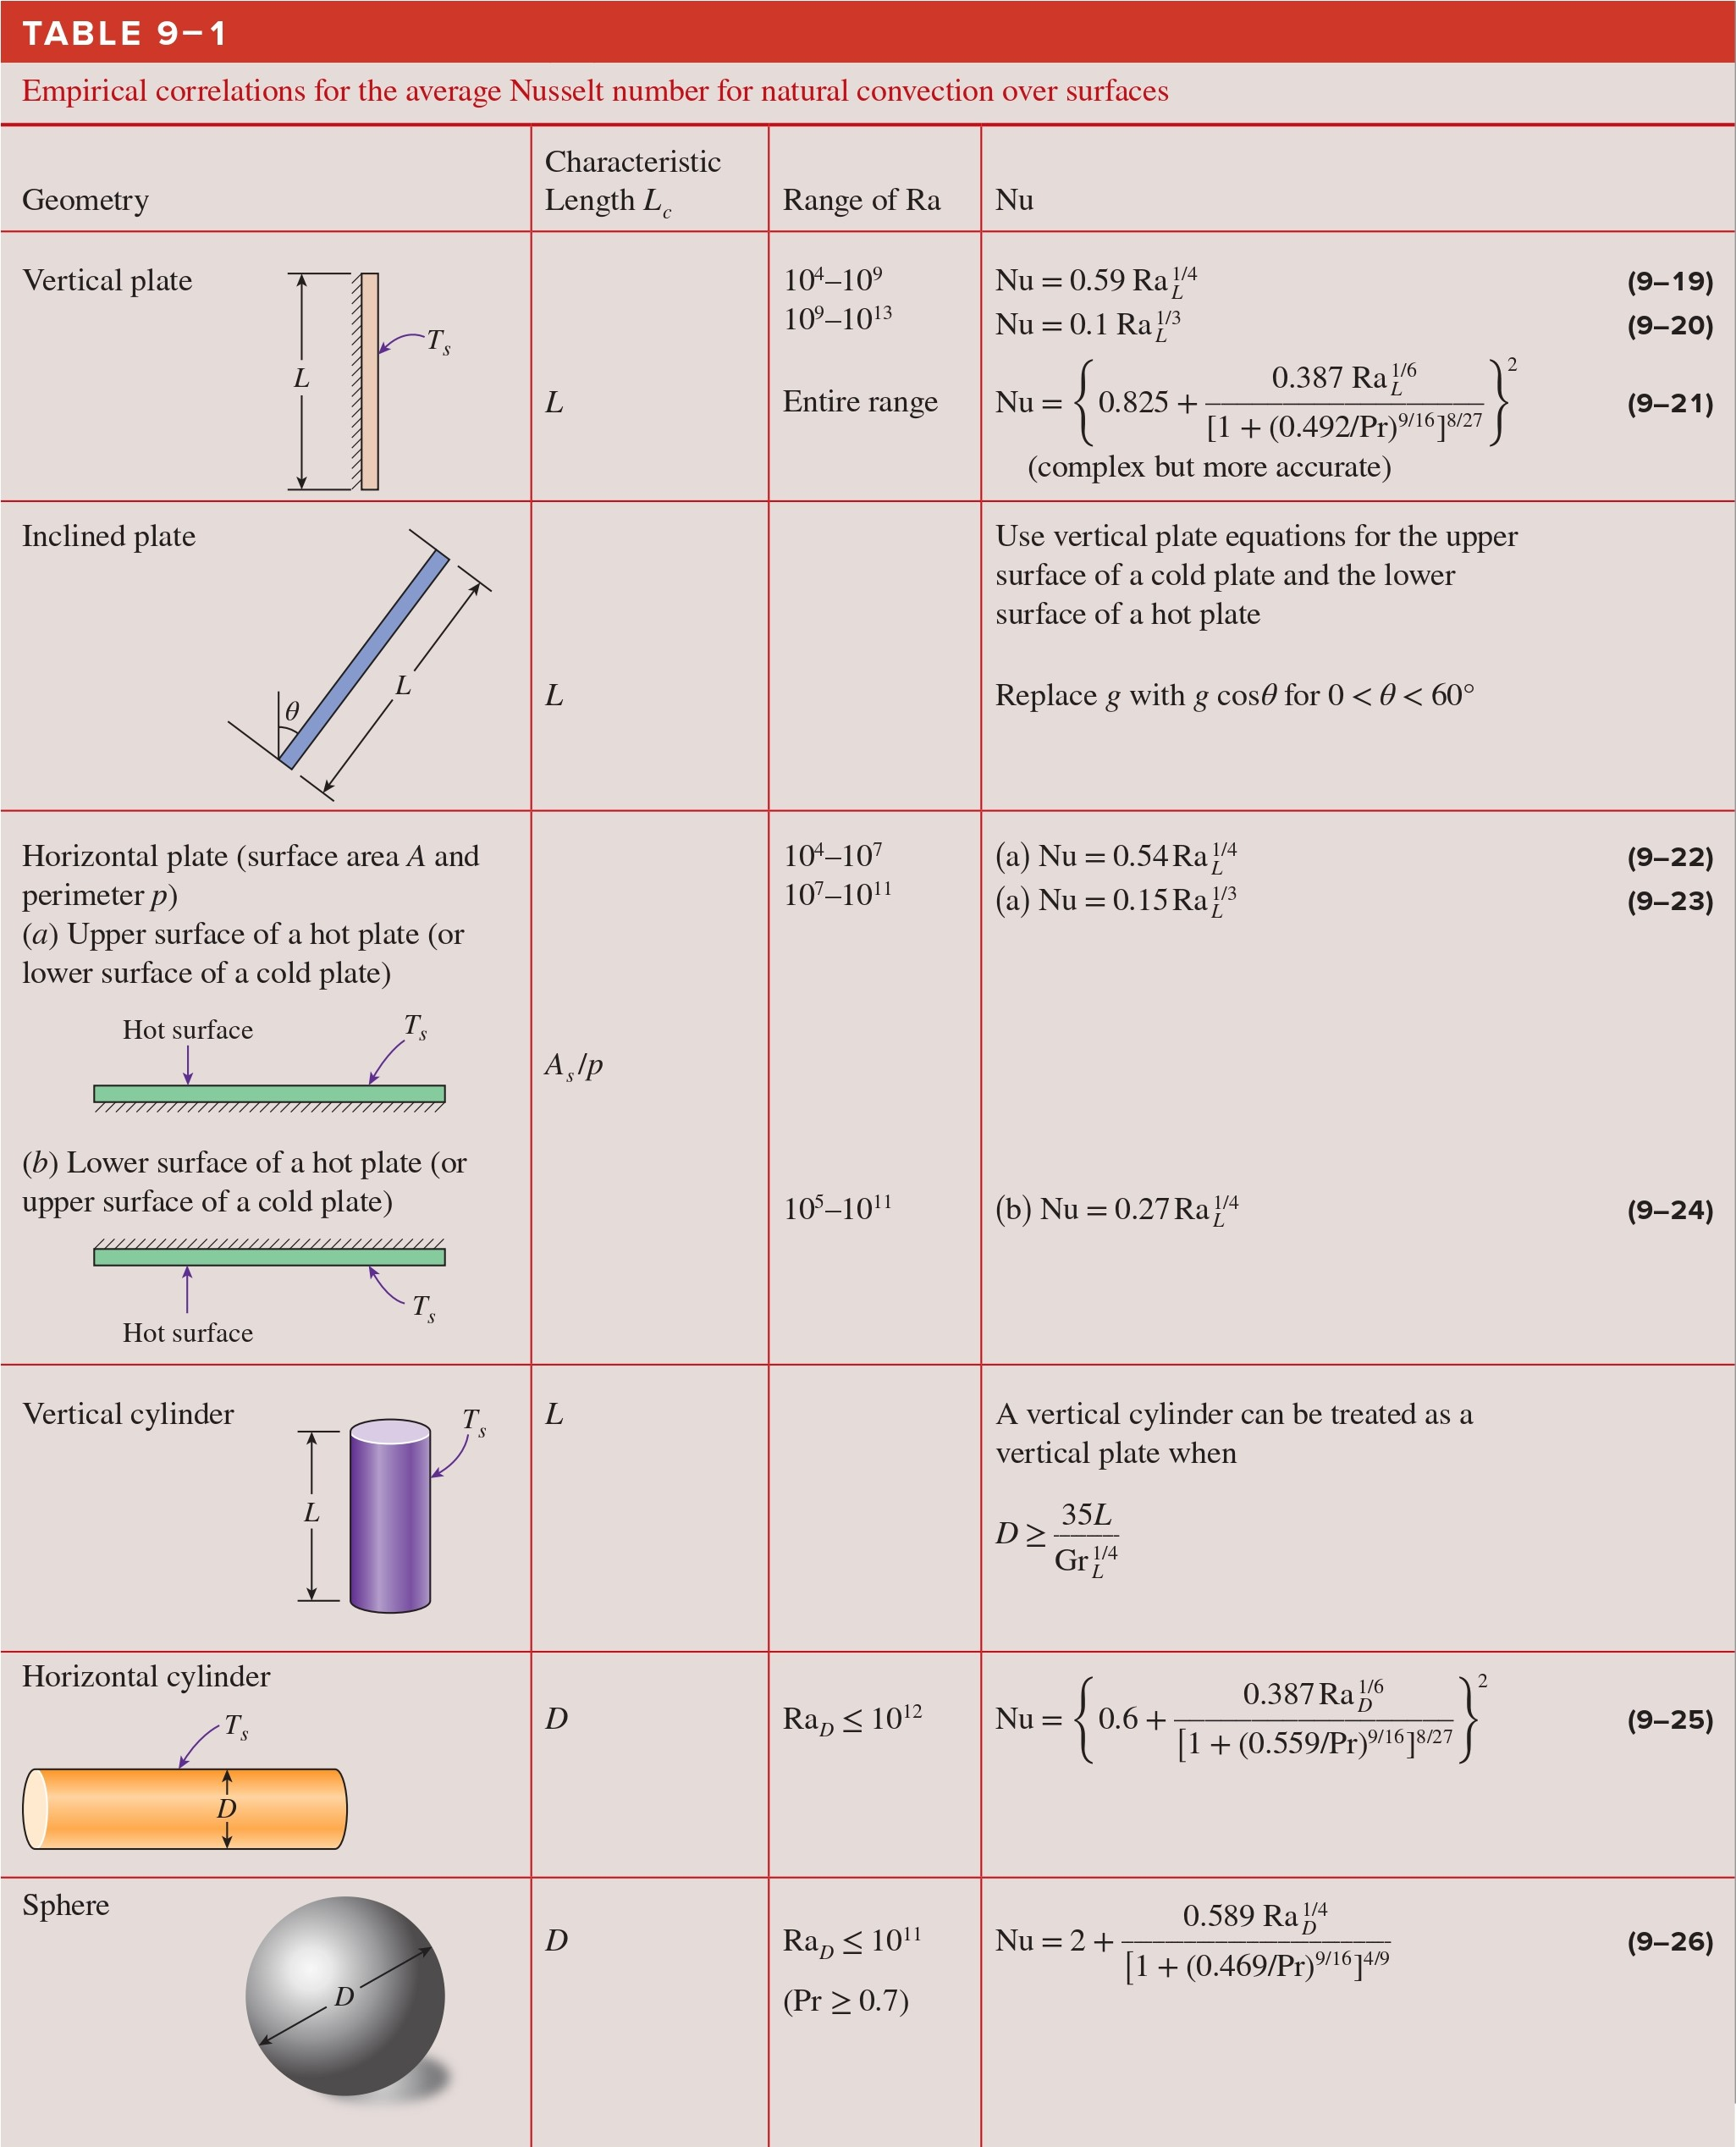
\includegraphics[width=0.8\textwidth]{Figures/sec9 table 9-1.jpg}
    \label{tab:sec9_natural_convection_over_surfaces}
\end{table}

% %     \centering
%     \caption{Nusselt number and friction factor for fully developed laminar flow in tubes of various cross sections 
%     ($D_h = 4A_c /P$, $Re = V_{\text{avg}} D_h / \nu$, and $\text{Nu} = hD_h / k$) (\textbf{Table 8-1 in textbook})}
%     \label{tab:sec8_fully_developed_laminar}
%     \begin{tabular}{ccccc}
%         \hline
%         & & \multicolumn{2}{c}{Nu} & \\
%         \cline{3-4}
%         Tube Geometry & $a/b$ or $\theta^\circ$ & $T_s = \text{constant}$ & $\dot{q}_s = \text{constant}$ & $f$ \\
%         \hline
%         \raisebox{-\totalheight}{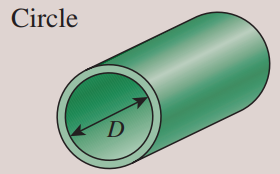
\includegraphics[width=0.15\textwidth]{Figures/Sec8 Circle Fully Laminar.png}} & --- & 4.36 & 3.66 & 64/Re \\
%         \hline
%         & \underline{$a/b$} & & & \\ 
%         \multirow{2}{*}{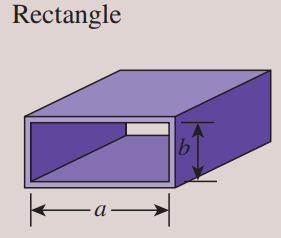
\includegraphics[width=0.15\textwidth]{Figures/Sec8 Rectangle Fully Laminar.png}} 
%         & 1 & 2.98 & 3.61 & 56.92/Re \\
%         & 2 & 3.39 & 4.12 & 62.20/Re \\
%         & 3 & 3.96 & 4.79 & 68.36/Re \\
%         & 4 & 4.44 & 5.33 & 72.92/Re \\
%         & 6 & 5.14 & 6.05 & 78.80/Re \\
%         & 8 & 5.60 & 6.49 & 82.32/Re \\
%         & $\infty$ & 7.54 & 8.24 & 96.00/Re \\
%         \hline
%         & \underline{$a/b$} & & & \\
%         \multirow{2}{*}{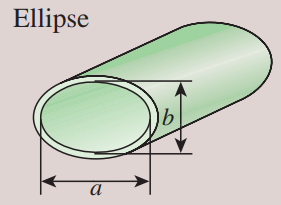
\includegraphics[width=0.15\textwidth]{Figures/Sec8 Ellipse Fully Laminar.png}}
%         & 1 & 3.66 & 4.36 & 64.00/Re \\
%         & 2 & 3.74 & 4.56 & 67.28/Re \\
%         & 4 & 3.79 & 4.88 & 72.96/Re \\
%         & 8 & 3.72 & 5.09 & 76.60/Re \\
%         & 16 & 3.65 & 5.18 & 78.16/Re \\
%         \hline
%         & \underline{$\theta^\circ$} & & & \\
%         \multirow{2}{*}{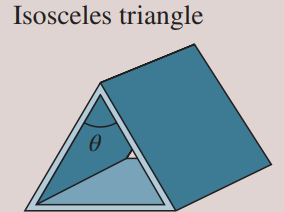
\includegraphics[width=0.15\textwidth]{Figures/Sec8 Triangle Fully Laminar.png}}
%         & 10 & 1.61 & 2.45 & 50.80/Re \\
%         & 30 & 2.26 & 2.91 & 52.28/Re \\
%         & 60 & 2.47 & 3.11 & 53.32/Re \\
%         & 90 & 2.34 & 2.98 & 52.60/Re \\
%         & 120 & 2.00 & 2.68 & 50.96/Re \\
%         \hline
%         % \raisebox{-\totalheight}{\includegraphics[width=0.15\textwidth]{Figures/Sec8 Square Fully Laminar.png}} & 1 & 3.66 & 3.11 & 64/Re \\
%     \end{tabular}
\newpage
\begin{multicols*}{2}
\section*{12. Thermal Radiation Fundamentals}
\subsection*{12.1. General Procedure}
Most questions will ask for irradiation given some geometry and temperatures.
\begin{enumerate}
    \item Determine absorptivity $\alpha$, reflectivity $\rho$, and transmissivity $\tau$ using the geometry and material properties. 
    Note that if two of these are known, the third can be found using $\alpha + \rho + \tau = 1$.
    \item Use solid angle $\omega$, irradiation $G$, and intensity $I$ to find whatever is asked for
\end{enumerate}
\subsection*{12.2. Variable Definitions}
\begin{itemize}
    \item $\omega$: Solid angle
    \item $G$: Irradiation
    \item $I$: Intensity
    \item $J$: Radiosity
    \item $\dot{Q}$: Heat transfer rate
    \item $\alpha$: Absorptivity
    \item $\rho$: Reflectivity
    \item $\tau$: Transmissivity
    \item $\epsilon$: Emissivity
    \item $\sigma$: Stefan-Boltzmann constant
\end{itemize}

\subsection*{12.3. Formulas}
For $A \ll r^2$ (small area, far away from surface),
\begin{align*}
    \omega_{2-1} &:= \frac{A_2 \cos\theta_2}{r^2}\\
    J_1 &:= \pi I_{1, e+r} = E_b + G_{\text{ref}} = \epsilon\sigma T_{1}^4  + \rho G_{1} \\ 
    \dot{Q}_{1-2} &:= I_1 (A_1 \cos\theta_1) \omega_{2-1} \\
    G_2 &:= \frac{\dot{Q}_{1-2}}{A_2} 
\end{align*}
Combining the above equations into $G_2$,
\begin{align*}
    G_2 &= \frac{(\epsilon\sigma T_{1}^4  + \rho G_{\text{1}})A_1 \cos\theta_1 \cos\theta_2}{\pi r^2} 
\end{align*}
For $\theta_1 = \theta_2 = \rho = 0$ and $\epsilon = 1$ for a blackbody,
\begin{align*}
    G_2 &= \frac{\sigma T_{1}^4 A_1}{\pi r^2} \\
    \implies T_{1} &= \left(\frac{G_2 \pi r^2}{\sigma A_1}\right)^{1/4}
\end{align*}

\end{multicols*}
\newpage
\begin{multicols*}{2}
\section*{13. Thermal Radiation Heat Transfer}
\subsection*{13.1. General Procedure}
Most questions will ask for irradiation given some geometry and temperatures.
\begin{enumerate}
    \item Determine view factors $F_{ij}$ from inspection using the geometry.  Check for special cases such as:
    \begin{itemize}
        \item $F_{ii} = 0$ when the surface $i$ is planar or convex
        \item $F_{ij} = 1$ when the surface $i$ is a concave and fully encloses surface $j$
    \end{itemize}
    \item Check Figures section for view factors that cannot be obtained from inspection
    \item Use the reciprocity relation and summation rule to find the remaining view factors
\end{enumerate}
Solvability condition: Given $N$ surfaces, there are $N^2$ view factors. $N(N-1)/2$ view factors must be 
given by inspection, problem statement, or tables. The rest can be determined using reciprocity and summation.
\subsection*{13.2. Variable Definitions}
\begin{itemize}
    \item $F_{ij}$: View factor, the fraction of radiation leaving surface $i$ that strikes surface $j$ 
    \item $\omega$: Solid angle
    \item $G$: Irradiation, the rate of radiant energy incident on a surface per unit area
    \item $I$: Intensity
    \item $J$: Radiosity, the total rate of radiant energy leaving a surface per unit area
    \item $E_{b}$: Black body emissive power
    \item $\dot{Q}$: Heat transfer rate
    \item $\alpha$: Absorptivity
    \item $\rho$: Reflectivity
    \item $\tau$: Transmissivity
    \item $\epsilon$: Emissivity
    \item $\sigma$: Stefan-Boltzmann constant
\end{itemize}
\subsection*{13.3. Formulas}
Reciprocity relation:
\begin{align*}
    A_{1, s} F_{12} &= A_{2, s} F_{21} 
\end{align*}
Summation rule:
\begin{align*}
    \sum_{j=1}^n F_{ij} &= 1 
\end{align*}
Crossed-strings method:
\begin{figure}[H]
    \centering
    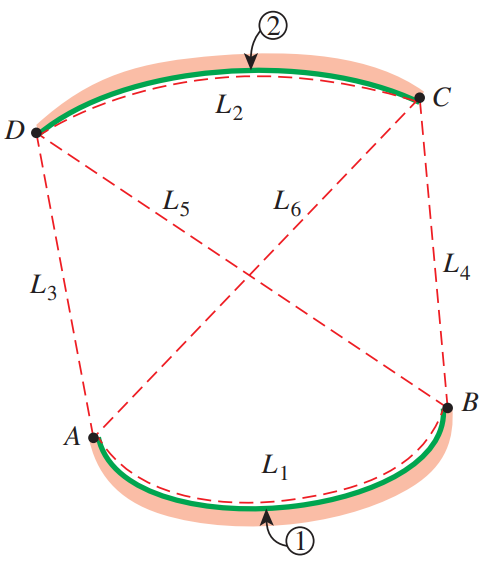
\includegraphics[width=0.2\textwidth]{Figures/Sec13 crossed strings.png}
    \caption{Determination of the view factor $F_{12}$ by the application of the crossed-strings method.}
    \label{fig:sec13_crossed_strings}
\end{figure}
\begin{align*}
    F_{12} &= \frac{(L_5 + L_6) - (L_3 + L_4)}{2 L_1} 
\end{align*}
On a black body, net radiation heat transfer is
\begin{align*}
    E_{bi} &= \sigma T_i^4 \\
    \dot{Q}_{12} &= A_{1, s} F_{12} \sigma (T_1^4 - T_2^4) = A_{2, s} F_{21} \sigma (T_1^4 - T_2^4) 
\end{align*}
On a grey body ($\epsilon_i = \alpha_i$, $\tau = 0$, $\alpha_i + \rho_i =1$), net radiation heat transfer is
\begin{align*}
    J_i &= \pi I_i = \epsilon_i \sigma T_i^4 + \rho_i G_i \\
    \dot{Q}_{12} &= \frac{A_{i, s} \epsilon_{i}}{1 - \epsilon_i} (E_{bi} - J_i) 
\end{align*}
For radiation in two-surface enclosures, net radiation heat transfer is
\begin{align*}
    \dot{Q}_{12} &= \dot{Q}_{1} = -\dot{Q}_{2} \\
    \dot{Q}_{12} &= \frac{\sigma (T_{1}^4 - T_{2}^4)}{\frac{1- \epsilon_1}{\epsilon_1 A_{1, s}} + \frac{1}{A_{2, s} F_{12}} + \frac{1-\epsilon_2}{\epsilon_2 A_{2, s}}} \\
    &= \frac{E_{b1} - E_{b2}}{R_{1} + R_{12} + R_{2}} 
\end{align*}
For some familiar geometries, the above equation simplifies, which is given in Table \ref{tab:sec13_radiation_enclosure_relations}.
\end{multicols*}

\section*{Figures}
\label{sec:sec13_figures}
\begin{figure}[H]
    \centering
    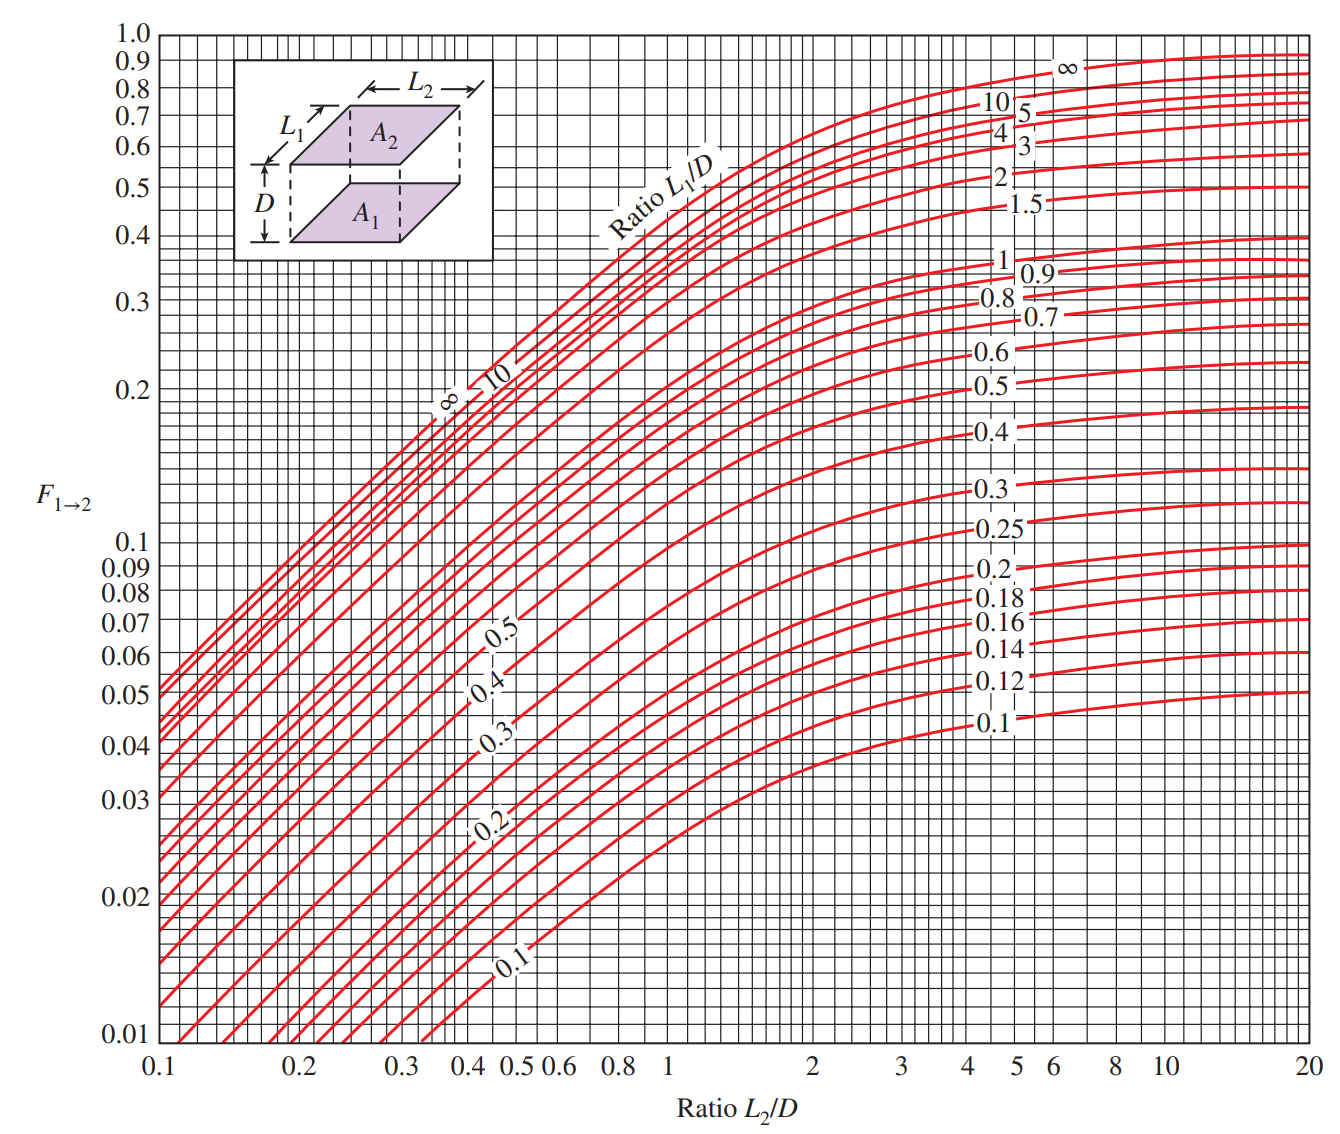
\includegraphics[width=0.6\textwidth]{Figures/Sec13 aligned parallel plates.png}
    \caption{View factor between two aligned parallel rectangles of equal size}
    \label{fig:sec13_aligned_parallel_rectangles}
\end{figure}
\begin{figure}[H]
    \centering
    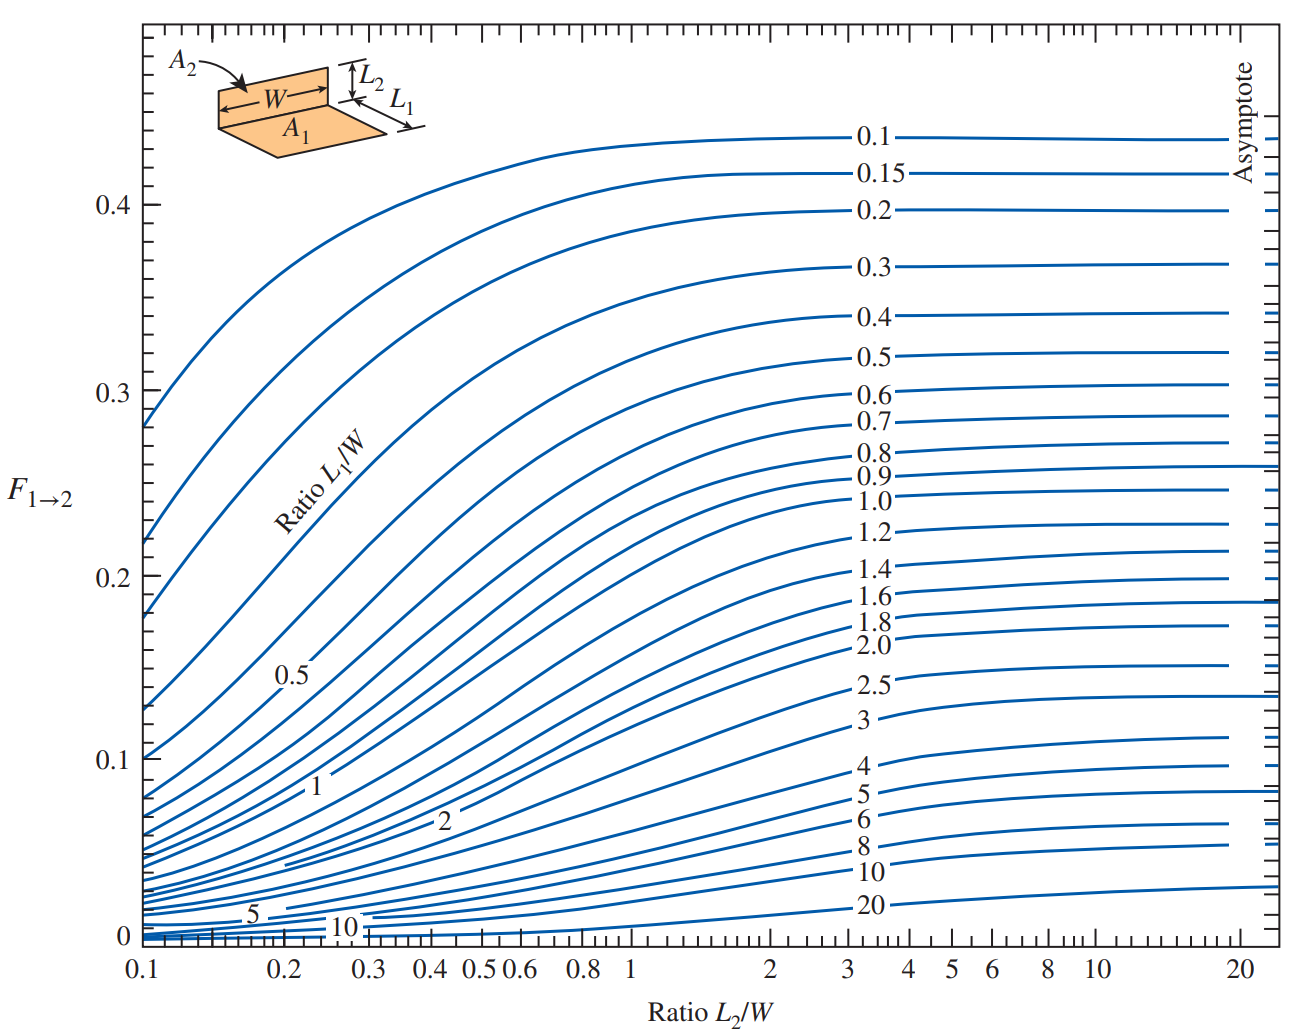
\includegraphics[width=0.6\textwidth]{Figures/Sec13 perpendicular rectangle.png}
    \caption{View factor between two perpendicular rectangles with a common edge}
    \label{fig:sec13_perpendicular_rectangles}
\end{figure}
\begin{figure}[H]
    \centering
    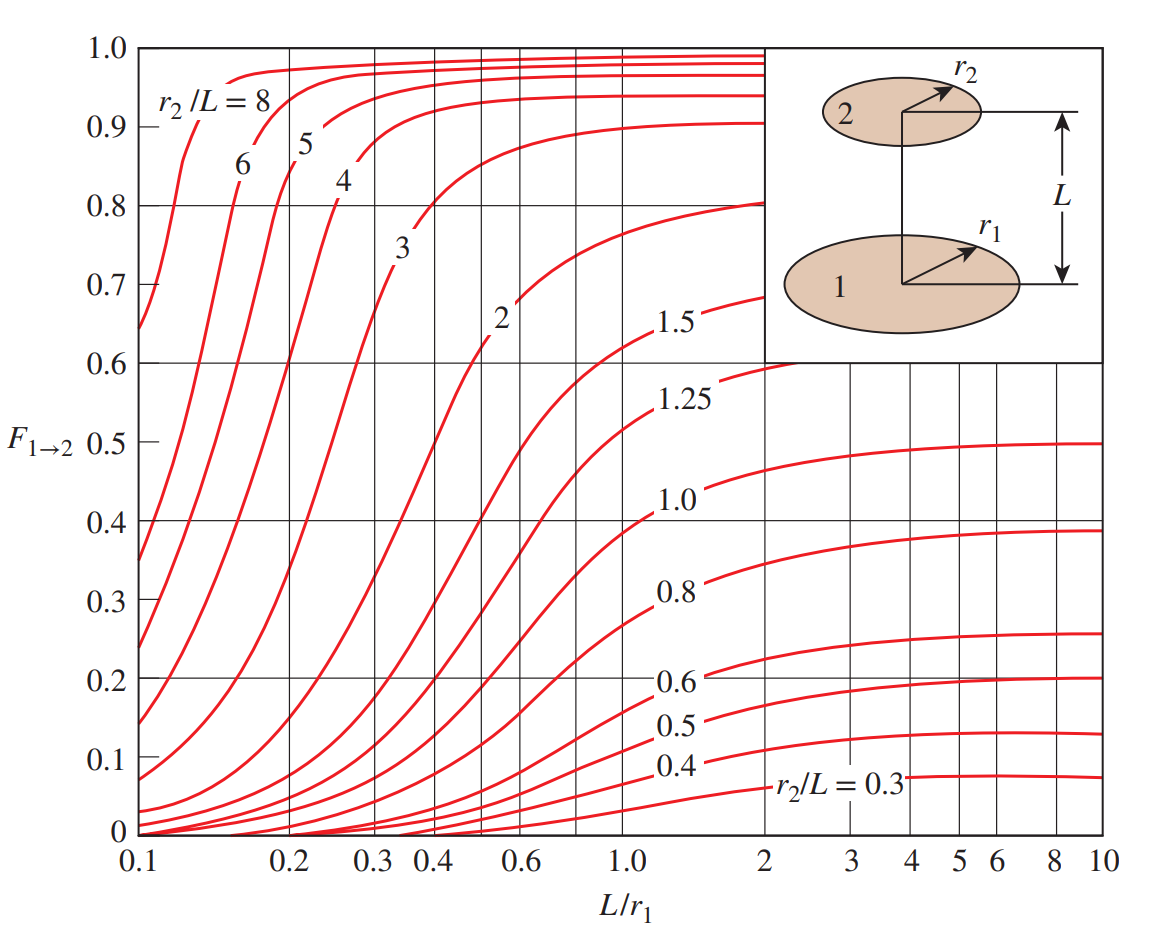
\includegraphics[width=0.6\textwidth]{Figures/Sec13 coaxial parallel disk.png}
    \caption{View factor between two coaxial parallel disks}
    \label{fig:sec13_coaxial_parallel_disks}
\end{figure}
\begin{figure}[H]
    \centering
    \begin{subfigure}[b]{0.4\textwidth}
        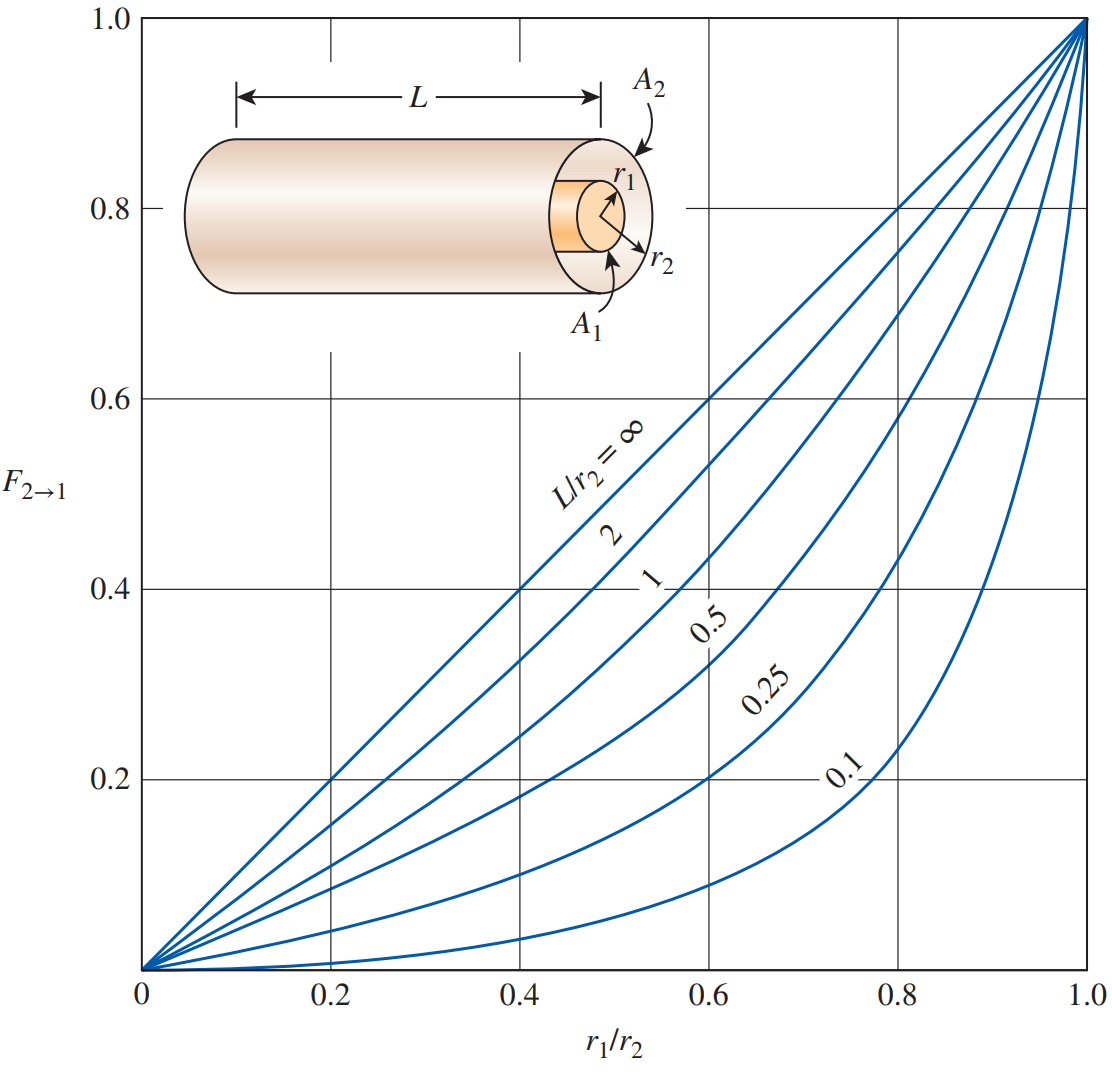
\includegraphics[width=\textwidth]{Figures/Sec13 concentric 2-1.png}
    \end{subfigure}
    \begin{subfigure}[b]{0.4\textwidth}
        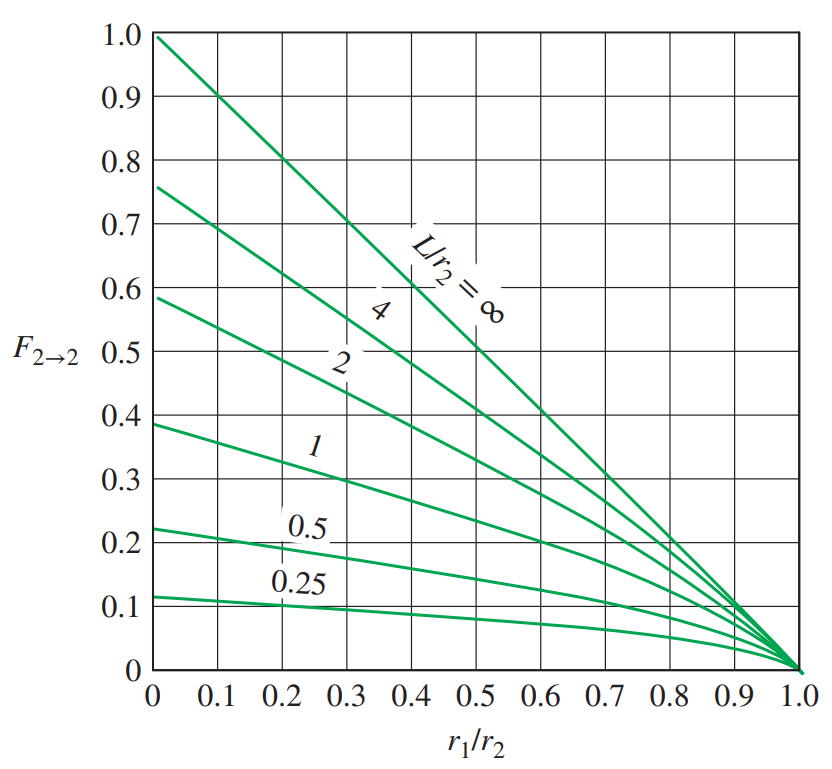
\includegraphics[width=\textwidth]{Figures/Sec13 concentric 2-2.png}
    \end{subfigure}
    \caption{View factors for two concentric cylinders of finite length: (a) outer cylinder to inner cylinder; (b) outer cylinder to itself.}
    \label{fig:sec13_concentric_cylinders}
\end{figure}

\section*{Tables}
\begin{table}[H]
    \centering
    \caption{Radiation heat transfer relations for some familiar two-surface arrangements}
    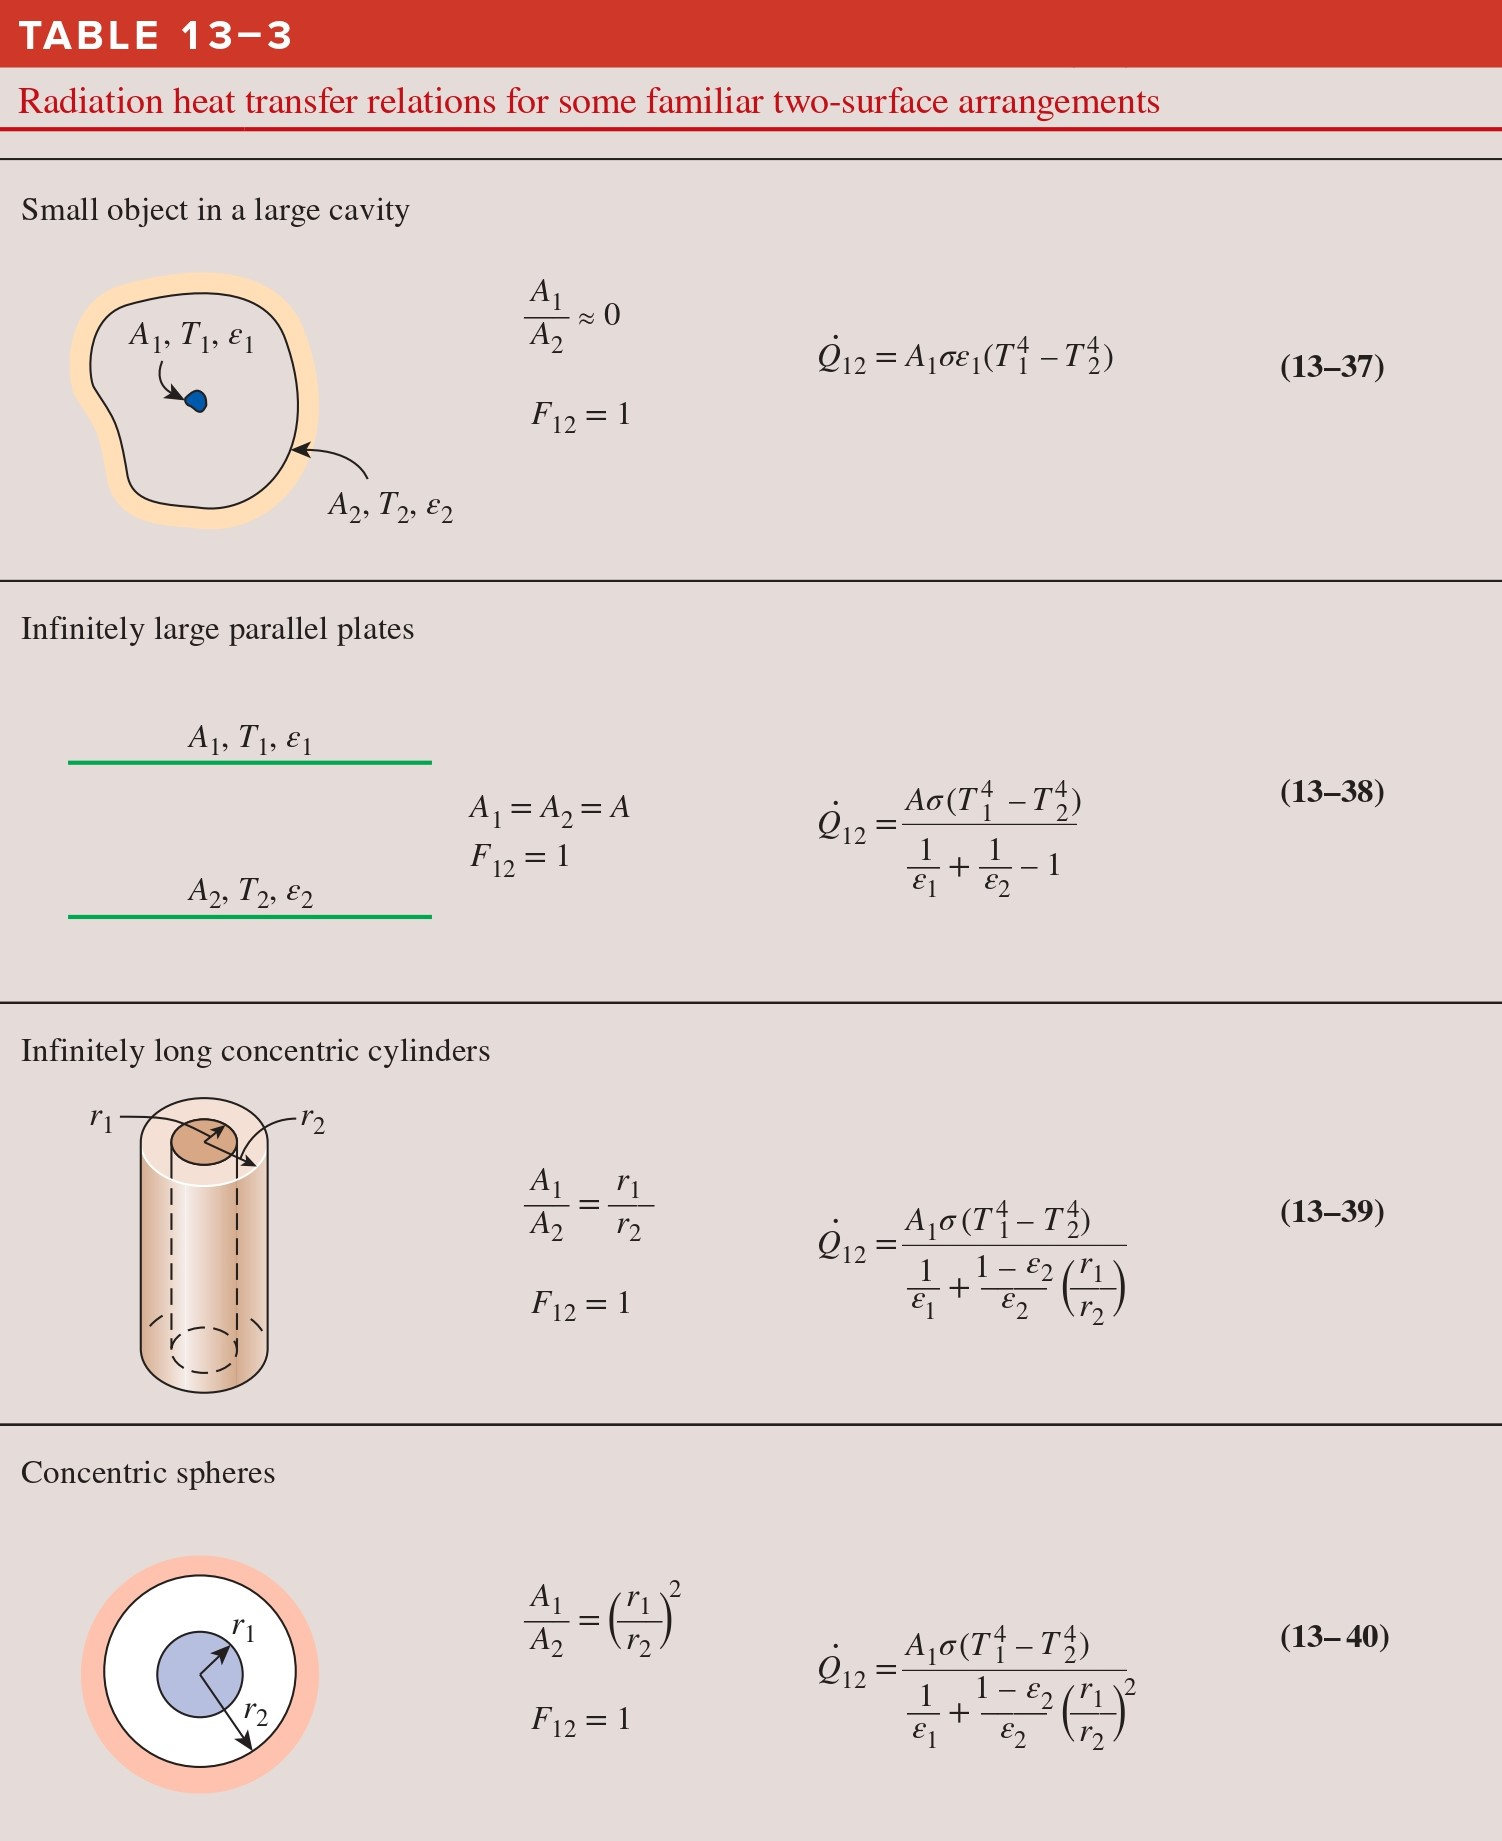
\includegraphics[width=0.8\textwidth]{Figures/Sec13 heat transfer enclosed.png}
    \label{tab:sec13_radiation_enclosure_relations}
\end{table}

\end{document}
